%
% Vorlage Diplom-/Master-/Bachelorarbeit
% Norman Heino
% Version: 0.1
% Datum: 2011-03-16
% Encoding: UTF-8
%
\documentclass[% 
  parskip=half,
  ]{scrreprt} % 11pt is default

\usepackage[automark, headsepline]{scrpage2}
%\usepackage{Sweave}
%\usepackage{showframe}
\usepackage[justification=centering]{caption}
\pagestyle{scrheadings}

% Kolumnentitel in Serifenloser Schrift
\renewcommand*{\headfont}{\normalfont\sffamily\slshape}

% Alle Seiten sind rechte Seiten
\refoot[\pagemark]{\pagemark}
\rofoot[\pagemark]{\pagemark}
\rehead[]{\headmark}
\rohead[]{\headmark}
\chead[]{}
\cfoot[]{}

% „--“ zwischen Kapitel und Kolumnentitel
\renewcommand*{\chaptermarkformat}{%
  \chapappifchapterprefix{\ }
  \thechapter\autodot\enskip{--}\enskip%
}

% Use utf-8 encoding for foreign characters
\usepackage[utf8]{inputenc}

% Fonts
% Roman
\usepackage[sc]{mathpazo}
% Sans
\usepackage{avant}
% \usepackage[scaled=.95]{helvet}

% Monospaced
\usepackage[scaled=.86]{beramono}
% Mono aus den pxfonts
% \renewcommand{\ttdefault}{pxtt}
% \DeclareMathAlphabet{\mathtt}{OT1}{pxtt}{m}{n}
% \SetMathAlphabet{\mathtt}{bold}{OT1}{pxtt}{b}{n}

% Support for multiple languages
\usepackage[english,ngerman]{babel}

% Non-english bibliography
\usepackage[fixlanguage]{babelbib}
\selectbiblanguage{ngerman}

% Nicer looking fonts
\usepackage[T1]{fontenc}

% Farben
\usepackage{color}

% Conditionals
% See ftp://ftp.rrzn.uni-hannover.de/pub/mirror/tex-archive/macros/latex/contrib/xifthen/xifthen.pdf
\usepackage{xifthen}

% This is now the recommended way for checking for PDFLaTeX:
\usepackage{ifpdf}

% Document info vars
\newcommand{\diplfirstname}{Marcus}
\newcommand{\diplname}{Nitzschke}
\newcommand{\dipltitle}{Patient-centered Drug Management based on Linked Open Data}
\newcommand{\diplsubtitle}{(Arbeitstitel)}
\newcommand{\diplsubject}{Master's Thesis}

\definecolor{remcolor}{rgb}{.95,0.35,0.35}

\newcommand{\rem}[1]{\textcolor{remcolor}{\emph{#1}}}

% Hyperref
\ifpdf
%\usepackage[pdftex]{graphicx}
\usepackage[
  pdftex, 
  pdfpagelabels,
  colorlinks=false,
  pdfborder={0 0 0},
  pdftitle={\dipltitle: \diplsubtitle},
  pdfauthor={\diplfirstname\ \diplname},
  pdfsubject={\diplsubject},
  pdfkeywords={}]{hyperref}
\else
\usepackage{graphicx}
\fi

\usepackage{graphicx}
\usepackage{epstopdf}
\usepackage{listings}
\usepackage{color}
\usepackage{url}
\usepackage{booktabs}
\usepackage{multirow}
\usepackage{rotating}
\usepackage{mathtools}

% Abbreviations
\newcommand{\linenumberstyle}{\scriptsize}
\newcommand{\lla}{\ensuremath{\longleftarrow}}
\newcommand{\todo}[1]{\marginline{\footnotesize TODO: #1}}
\newcommand{\pdfscale}{1.0} % Global scaling factor for included PDF files
\newcommand{\enlarge}{\enlargethispage{1.5em}}

% Adapt LaTeX defaults
\linespread{1.4}
\setlength{\abovecaptionskip}{.5em}
\setlength{\parindent}{1em}
\setlength{\parskip}{.2em}

% continous footnotes
\usepackage{remreset}
\makeatletter
\@removefromreset{footnote}{chapter}
\makeatother

% Adapt KOMA defaults
\setcapindent{\parindent}
\setkomafont{captionlabel}{\sffamily\bfseries}


% Listings setup
% See http://ftp.fernuni-hagen.de/ftp-dir/pub/mirrors/www.ctan.org/macros/latex/contrib/listings/listings.pdf

% define json listings
\lstdefinelanguage{json} {
  sensitive=false, 
  morestring=[b]"', 
  showstringspaces=false
}

% define turtle listings
\lstdefinelanguage{turtle} {
  sensitive=false, 
  morestring=[b]"', 
  showstringspaces=true
}

% define sparql listing
\lstdefinelanguage{sparql} {
  sensitive=false, 
  morestring=[b]"', 
  showstringspaces=true,
  backgroundcolor=\color[gray]{1.0},
  numbers=none,
  xleftmargin=0pt,
  xrightmargin=0pt,
  framexleftmargin=0pt,
  framexrightmargin=0pt
}

% set default listing style
\lstset{
  language=json, 
  basicstyle=\small\ttfamily, 
  captionpos=b, 
  % keywordstyle=\color[rgb]{0,0,0.7}, 
  % stringstyle = \color[rgb]{0,0.5,0}, 
  % identifierstyle=\color{orange}, 
  commentstyle=\color[gray]{0.5}, 
  backgroundcolor=\color[gray]{0.96}, 
  framexleftmargin=1pt,
  xleftmargin=4.4pt,
  xrightmargin=3.4pt,
  numbers=left, 
  numberstyle=\linenumberstyle, 
  frame=single, 
  aboveskip=1.3em
}

% Algorithms
% See ftp://ftp.tu-chemnitz.de/pub/tex/macros/latex/contrib/algorithm2e/algorithm2e.pdf
% \usepackage[german, algochapter, boxed, linesnumbered, vlined]{algorithm2e}
% \SetAlCapSkip{.885em}
% \SetNlSkip{1.5em}
% \SetInd{.8em}{.8em}
% \SetNlSty{linenumberstyle}{}{}
% \newcommand{\captionlabel}{\usekomafont{captionlabel}}
% \SetAlTitleFnt{captionlabel}

% Document info
\titlehead{
  \begin{center}
    \textsc{Universität Leipzig}\\
    Faculty of Mathematics and Computer Science\\
    Department of Computer Science
  \end{center}
}

% Generates the title
\title{%
\dipltitle\\%
\bigskip\usekomafont{subtitle}%
\parbox[h]{0.8\textwidth}{\begin{center}\diplsubtitle\end{center}}%
}

% Subtitle is abused as type of work
\subtitle{\usekomafont{subject}\vspace{3em}\diplsubject}
\author{}
\date{}
\publishers{
  \large\parbox{\textwidth}{%
    % \vspace*{4\baselineskip}
    Leipzig, March 2013\hfill 
    Submitted by\\
    \raggedleft
    \diplname, \diplfirstname\\
    Studiengang Informatik
  }\\
\raggedright
\vspace{2.5cm}
\textbf{Thesis Supervisors:\\
  Prof. Dr. Klaus-Peter Fähnrich\\
  Dipl. Inf. Romy Elze
  %Department of Computer Science
}
}

\begin{document}
\selectlanguage{english}

\ifpdf
\DeclareGraphicsExtensions{.pdf, .png, .jpg, .tif}
\else
\DeclareGraphicsExtensions{.eps, .jpg}
\fi

% Seitennummerierung auf römisch
\pagenumbering{roman}

% Titelei
\maketitle

\section*{Abstract}
This thesis will present a solution for a simple way to answer several drug related questions, like ``What are the side effects of drug X?'' or ``Do drug X and drug Y interact with each other?''.
The knowledge foundation used for these queries are Linked Data knowledge bases which allow comprehensive queries over semantic data.
The presented approach provides an Application Programming Interface (API) for the different questions that allows an usage without any background knowledge about the data sources and their structures.
Additionally the predefined questions support the ``Drug Management life cycle'' introduced by the World Health Organization.
Finally the presented solution will be evaluated by integrating it in the Dispedia and DrugMan project.

%%% Local Variables: 
%%% mode: latex
%%% TeX-master: "thesis"
%%% End: 

% Zusammenfassung
%\thispagestyle{empty}


\paragraph{Keywords} LinkedOpenData drug interaction Dispedia

% Verzeichnisse
\setcounter{tocdepth}{1}
\tableofcontents

% Ab nächster Seite
\clearpage
% Seitennummerierung auf arabisch
\pagenumbering{arabic}

% \begin{abstract}
% \end{abstract}

\chapter{Introduction}
\label{cha:introduction-1}

\section{Subject}
\label{sec-1}

\begin{itemize}
\item verschiedene anwendungen im  bereich arzneimittelmngtm
\item überschneidende funktionalität
\item 
\item keine endanwendungen auf lodd basierend bekannt
\end{itemize}
\section{Problem}
\label{sec-2}

\begin{itemize}
\item unterschiedliche implementierungen
\item unters. quellen
\item ausgesagt werden soll aber das selbe
\item 
\item umfangreiches schemawissen nötig um anfragen an lod stellen zu können
\end{itemize}
\section{Motivation}
\label{sec-3}

\begin{itemize}
\item durch einheitliche schnittstelle soll datenqualität vereinheitlicht werden
\item einstiegsbarriere für neue anwendunge senken (cpoe)
\item 
\item vereinfachen der möglichkeit wissen aus lodd zu nutzen
\item (praxiseinsatz von lodd)
\end{itemize}
\section{Objectives}
\label{sec-4}

\begin{itemize}
\item bereitstellen einer API zur unterstützung des drug management life cycles basierend auf lod(d)
\item evaluation anhand verschiedener anwendungsfälle
\begin{itemize}
\item dispedia
\item eigenes portal zur arzneimittel-verwaltung
\end{itemize}
\end{itemize}

%%% Local Variables: 
%%% mode: latex
%%% TeX-master: "../thesis"
%%% End: 


\chapter{Preliminaries}
\label{cha:prelims}

\section{Drug Management}
\label{sec:drug-management}
\begin{itemize}
\item abgrenzung zu klinischen drug management
\item who life cycle
\end{itemize}

\section{Semantic Web}
\label{sec:semantic-web}

\section{Linked Open Data}
\label{sec:linked-open-data}

%%% Local Variables: 
%%% mode: latex
%%% TeX-master: "../thesis"
%%% End: 


\chapter{Methods}
\label{cha:methods}

\begin{itemize}
\item sparql federated queries nicht überall unterstützt -> construct und dann lokales mergen
\end{itemize}



\chapter{Evaluation}
\label{cha:evaluation}

The evaluation of SEDRI has the goal to test how well it can be integrated in different projects with different use cases, based on different programming languages and so on.
This thesis will evaluate SEDRI by integrating it in two projects: Dispedia and DrugMan.

\section{Dispedia}
\label{sec:dispedia}
% \begin{itemize}
% \item Anwendungsfälle und Vorgehen beschreiben
% \end{itemize}

\subsection{Introduction}
\label{sec:introduction}
% \begin{itemize}
% \item konzept prop, propcomp
% \item patient medikationsplan
% \item unterscheidung drug/drug product
% \end{itemize}

``The Dispedia Framework is an information system in the complex field of rare diseases. The goal of the system is to harmonize social care conditions and health care conditions with the focus on personalization and patient autonomy.'' \cite{elze2013dispedia}\\
Dispedia is based on several ontologies and uses Linked Open Data e.g. for additional information about diseases or drugs.
The following paragraph will describe some of the core concepts of Dispedia which are essential for the integration of SEDRI.

Maybe the most important core concept are \textit{Proposals}.
A proposal is a possibility of a physician to offer several therapeutical activities to a patient.
In the Dispedia model a proposal represents a frame for multiple proposal components.
A proposal component in turn contains the mentioned therapeutical activities like prescribing drugs, medical devices or other services.
Proposal components act like bricks which can be assigned to different proposals.
This is a flexible way to create treatment offers.
Proposals are assigned to patients.
The relationship proposal -- patient is $n:m$ which means that it is possible to assign a proposal to multiple patients and that a patient can hold multiple proposals.\\
Besides these proposals a patient can receive several products or services, like drug products or a physiotherapy.
This is relevant for the integration of SEDRI because in that way there are two ways how a patient can take drugs.
First by accepting a proposal and second by ``receiving'' a drug product on their own.\\
The third important concept is the distinction between a drug and a drug product.
As described in the last sentences a patient can receive a drug product.
A drug product is a concrete commercial product distributed by a pharma company.
These products include an active ingredient which is the ``drug'' in the Dispedia sense.
An example of the distinction may be the drug product ``Ibuflam'' and the drug ``Ibuprofen''.

\subsection{Integration of SEDRI}
\label{sec:integration-sedri}

The integration point of SEDRI in Dispedia is the possibility to propose a specific drug to a patient.
In that case SEDRI is used to check the proposed drugs for possible drug-drug interactions.
In detail there are three integration points which are described in the following listing in more detail: 
\begin{itemize}
\item \textit{Check A}: The first integration is when a proposal component is created.
Each proposal component can contain multiple drugs.
If such a proposal component is created or modified then the containing drugs are tested for possible interactions.
In this case Dispedia has nothing to do than calling SEDRI with the appropriate drug codes that are stored in the system and to process the results.
\item \textit{Check B}: The second integration is implemented in the logic of proposals.
As the introduction about Dispedia described each proposal can contain multiple proposal components which thereself contains drugs.
In this scenario it is possible that a physician proposes a specific proposal including multiple components where each component itself contains no interactions but the components among each other contains interactions.
To prevent such a scenario the components of a proposal are tested for interactions on creation and modification of the proposal.
\item \textit{Check C}: The third integration of the drug-drug interaction endpoint is implemented in the patient proposal allocation.
If a physician allocates several proposals to a patient, these proposals will be checked against the current medication of the patient.
This prevents patients to get interacting drugs in their medication plan.
In this third case one difference to the other two implementations has to be considered.
Because the items of the medication plan of the patient are drug products in the meaning of Dispedia the active ingredient of this drug product has to be received.
In the other two cases the drugs could be directly compared because the proposals and proposal components contain no drug products but drugs.
\end{itemize}
If in one of those cases an interaction is detected the details of the interaction are saved in relationship to the corresponding instance of the proposal or proposal component.
This allows the system to provide these information in other use cases.
For example when a patient decides to accept or decline a proposal the possible interaction information of the third check can be provided.
In this case an additional call of SEDRI is not necessary.

\begin{figure}
  \centering
  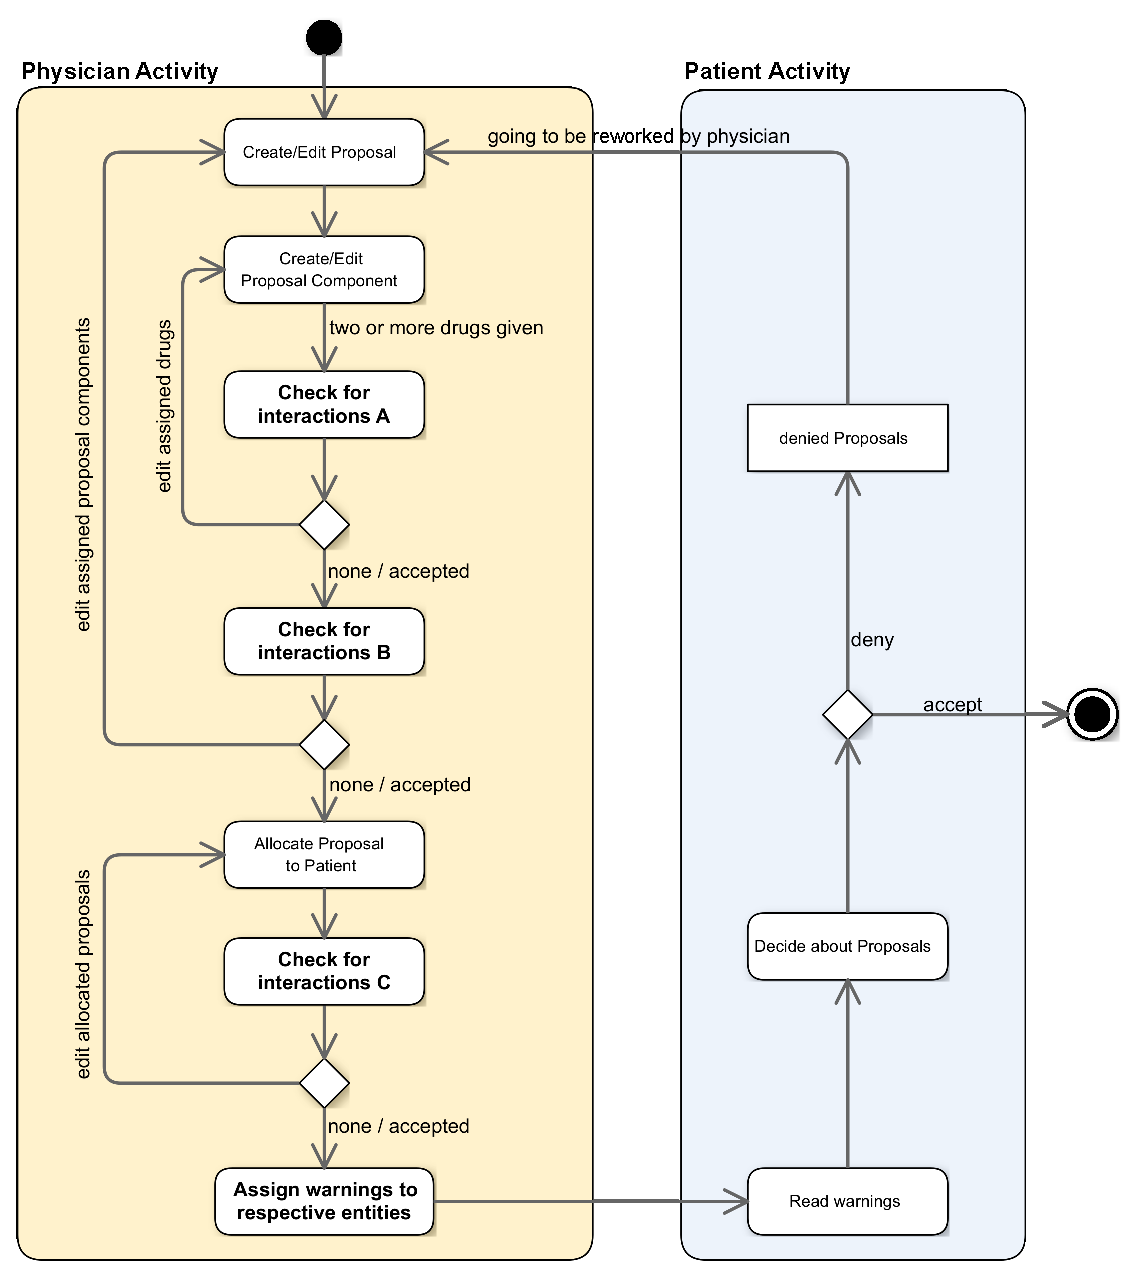
\includegraphics[scale=0.49]{evaluation/Dispedia_Integration_activity}
  \caption{Activity diagram of Dispedia proposal workflow}
  \label{fig:dispedia_activity}
\end{figure}
Figure \ref{fig:dispedia_activity} gives a graphical overview of the typical proposal workflow in Dispedia and where SEDRI is used.\todo{grafik}\\
The workflow is divided in the physician's activity and the patient's activity.
The beginning of the workflow is the creation of a new proposal by a physician.
If there are already existing proposal components then several of these components can be added to the new proposal.
Otherwise or additionally it is possible to create new proposal components.
These proposal components may contain drugs or other therapeutical activities as described in the previous introduction section.
If a new proposal component was created the included drugs will be tested for drug-drug interactions by SEDRI (\textit{Check A}).
After all desired proposal components are added to the proposal and the proposal is saved, the second call of SEDRI (\textit{Check B}) is executed.
Now the new proposal can be allocated to several patients.
In this step SEDRI executes the third check (\textit{Check C}).
With the completed proposal allocation the activity of the physician is finished.
The patient's activity starts with taking note about the given drug-drug interactions in their allocated proposals.
Based on these information the patient can accept or decline a given proposal.
In case of accepting the proposal the workflow ends.
Otherwise the physician is notified that a proposal has been declined and the physician is now able to rework the proposal.
This means the workflow starts the next iteration.

\begin{figure}
  \centering
  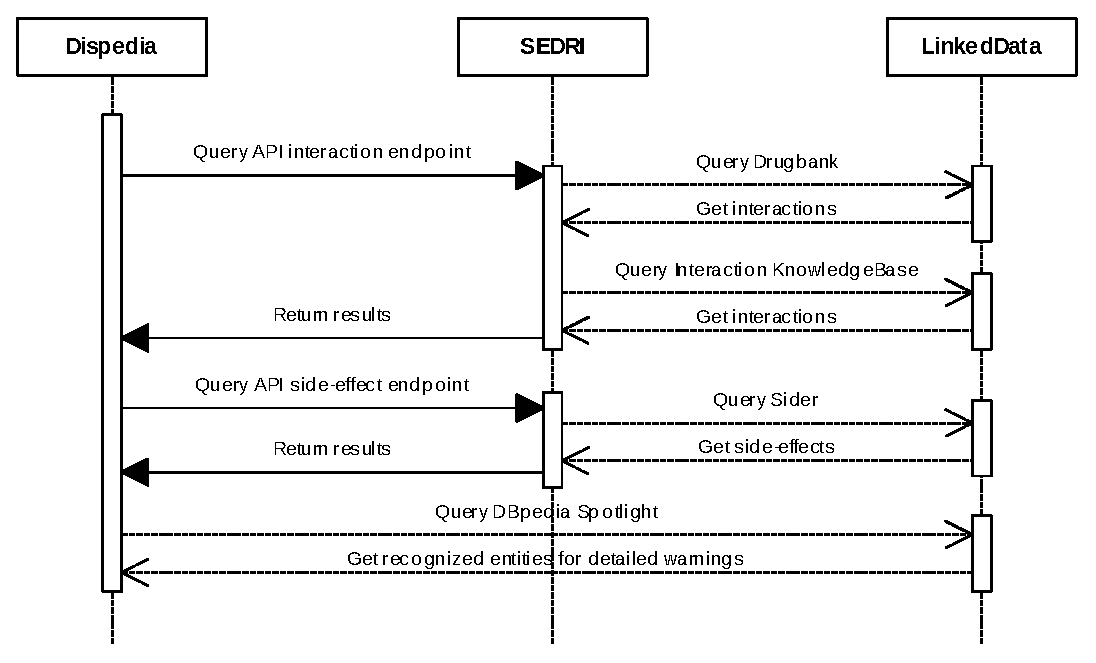
\includegraphics[width=\textwidth]{evaluation/LODD_Wrapper_Sequences.eps}
  \caption{Sequence diagram of Dispedia and SEDRI information flow}
  \label{fig:dispedia_sequence}
\end{figure}
Figure \ref{fig:dispedia_sequence} gives an overview of the information flow between Dispedia, SEDRI and the Linked Open Data cloud.
It illustrates how Dispedia is calling SEDRI for two use cases, interactions and side effects.
The latter one was not in the scope of this evaluation and is not implemented yet.
The calls to SEDRI are synchronous which means Dispedia has to wait until the results are delivered by SEDRI to work on further.
SEDRI itself calls different Linked Data sources asynchronously.
After the results are delivered by SEDRI, the diagram shows that Dispedia continues processing these results.
In this case Dispedia calls the DBpedia Spotlight annotation service\footnote{\url{http://dbpedia-spotlight.github.io/demo/} (last access Sept 09, 2013)} which extracts several entities from a given text and links them to their DBpedia resources.
This can improve the given warning messages by much more information.

\section{DrugMan}
\label{sec:portal}

\subsection{Motivation}
\label{sec-1}

Spoken for Germany there is a static rise in the last years of multiple morbidities of patients.
These often imply automatically that the regarding patient takes also multiple drugs.
In the case of five or more medications this is called \textit{Polypharmacy} \cite{montamat1992overcoming}.
Besides the fact of the multiple medications this term stands also for the unnecessary prescription of drugs which may lead to several issues.

A general issue of polypharmacy is that it is hard for patients as well as physicians or pharmacists to keep track of all the currently prescribed medications.
Additionally the patient can buy several prescription free drugs that also could lead to issues with the other prescribed drugs.
If this overview of all the medication can not be preserved then different physicians may prescribe independently their drugs what often leads to overlapping prescriptions or interacting drugs in the medication of the patient.

Another problem that DrugMan is facing is the low self-determination of people during pharmacotherapy.
This self-determination covers the confirmability and information procurement in the process of pharmacotherapy.
One example where these two values are lacking are drug-drug interactions.
If a patient is taking five drugs, which is the lower limit of polypharmacy, then there are ten possible drug-drug interactions that a patient has to test if he wants to know whether his medication includes interactions or not.
These information about possible interactions are provided by the instruction leaflet.
But these information -- in the case of Germany -- doesn't name any specific drug names but only drug classes.
So without any expert knowledge it is nearly impossible for a patient to get any concrete information about possible drug-drug interactions.
And in the case that the information would be available it is cumbersome for a private person to test all the possible combinations of drugs.
% \begin{itemize}
% % \item schwer für ärzte überblick über verfügbare medikamente am markt zu behalten
% % \item oft bilden sich aus erfahrung paare von medikamenten zu gegebener krankheit die nur selten dann erneuert werden (Quelle oä?)
% % \item 
% \item ärzte verschreiben oft unabhängig voneinander medikamente
% \item patient hat möglichkeit rezeptfreie medikamente zusätzlich einzunehmen
% \item bpz verweisen nur grob auf mögliche interaktionen
% \begin{itemize}
% \item oft nur gruppen von medikamenten genant, nicht medikamente konkret
% \end{itemize}
% \end{itemize}

% \begin{itemize}
% \item patienten bekommen arzneimittel verschrieben auf grund der erfahrung der ärzte nicht evidenzbasiert bzw. an aktuellen studien ausgerichtet
% \item mehr oder minder blindes vertrauen des patienten den ärzten gegenüber
% \item 
% \item bei n arzneimittel gibt es (n$^2$-n)/2 mögliche interaktionen
% \begin{itemize}
% \item 2->1, 3->3, 4->6, 5->10
% \end{itemize}
% \end{itemize}

% \begin{itemize}
% \item transparente möglichkeit der unterstützung von drug management eines patienten
% \item bereicherung der persönlichen freiheit durch nachvollziehbarkeit und kontrolle der eigenen arzneimitteltherapie
% \end{itemize}

\subsection{Features}
\label{sec:features}

Derived from the two problems described in the previous section, the goal of DrugMan -- a personal drug management portal -- is to provide a modern approach for supporting the patient during the pharmacotherapy.
This includes the possibility to capture the full medication of the patient and several actions that support the self-determination of the patient, e.g. testing the medication for drug-drug interactions.
DrugMan was developed as a side project of this thesis.
It therefore has a strong connection to SEDRI.\\
%The goal of this project is to support patients as well as private persons in managing their medications.\\
The following paragraphs will describe the core features of DrugMan.

\begin{figure}
  \centering
  \includegraphics[scale=0.38]{evaluation/drugman}
  \caption{Screenshot of DrugMan}
  \label{fig:drugman}
\end{figure}

% \subsubsection*{User management}
% DrugMan implements a classic user management approach.
% The registration is open for everyone
\subsubsection*{Medication plan}
The central part of DrugMan is the medication plan.
Each registered user can add several drugs to their medication plan.
This allows the user always to have the overview of the current taken drugs.
A drug item of the medication plan consists of a label and an active ingredient.

\subsubsection*{Drug details}
The details page about a drug gathers different information about the drug and their active ingredient.
One example for such details are pharmacokinetic information about the active ingredient. 
Among others these information contains the absorption, route of elimination and the affected organism.
Other examples for details are side effects or available packagers and manufacturers.

\subsubsection*{Interactions}
The first of several actions that can be executed on top of the medication plan is a drug-drug interaction check.
This action will test all the drugs that are included in the medication plan for possible drug-drug interactions.
These checks are based on the active ingredient of each drug.
In case of existing interactions the affected drug-drug combination and some details about the interaction will be communicated by a notification.

\subsubsection*{Side effect detector}
Another feature is the ``Side effect detector''.
By specifying several side effects, the side effect detector will return all the drugs of the medication plan that may cause these side effects.
The process of specifying the side effects is supported by an autocomplete function that gathers side effects from the SIDER knowledge base.
The matching is done by comparing the given side effect URI's of the user with all the URI's of possible side effects of the drugs inside the medication plan.

\subsubsection*{Drug proposals}
The drug proposal feature supports the user by informing about possible drugs to a given disease.
After specifying a disease the user will get a selection of possible drugs.
Based on this selection the user can read some details about the drug including side effects, add this drug to the medication list or check whether the drug suits to the other drugs of the medication list in terms of possible drug-drug interactions.

\subsection{Integration of SEDRI}
\label{sec-2}
Since DrugMan was developed as a side project of this thesis the project is tightly coupled with SEDRI.
The internal architecture of DrugMan can be grouped in the management component and the drug specific component.

The former one is responsible for the general management features like user management including registering new users, login, logout etc. and the medication plan features including the registration, modification and deletion of drug items.

The latter component is responsible for the drug-specific features and is completely based on SEDRI.
This means all the funtionality described in Section \ref{sec:features} except the medication plan is built on top of SEDRI.

An example that SEDRI is usable for frontend information as well as backend processing is the Side effect detector.
This feature uses the side effects endpoint of SEDRI in the backend for the internal comparison of the given side effects and all the possible side effects of the current medication.
On the other hand it uses the same endpoint in the frontend by displaying all available side effects in the detail page of a drug.

If desired the application could request different return formats for the different use cases.
But in the case of the Side effect detector JSON-LD is used for both processes and the evaluation showed that this suits well.
%%% Local Variables: 
%%% mode: latex
%%% TeX-master: "../thesis"
%%% End: 


\chapter{Summary}
\label{cha:summary}

This thesis presented an approach for answering several drug related questions based on Linked Open Data knowledge bases.
Section \ref{sec:objectives} stated the objective to provide an easy to use interface.
This objective could be achieved what is proofed by the evaluation projects.
Therefore the developers or later the respective users have nothing else to know than the appropriate drug names or drug codes.
All the required knowledge about the structure of the different knowledge bases is abstracted by SEDRI.
How easy the usage of SEDRI is showed the two evaluation projects.
They both showed also that SEDRI is usable independently of the programming language or other implementation details of the projects.
This is due to the integration and component characteristics of a web-based HTTP interface.
Thereby the two main objectives of section \ref{sec:objectives} are achieved.

The problems that were worked out in section \ref{sec:problem} could be avoided mostly by the infrastructure of SEDRI.
The first problem was insufficient integration which is mostly fixed by the Linked Data approach.
Having that said the integration could be further improved by implementing Entity Matching mechanisms or the like.
By using Linked Data as a knowledge foundation also the second problem -- redundancy -- is mostly fixed.
This is due to the several domain specific knowledge bases where only a small part of the data is redundant.
The last problem of possibly incorrect data is rather not applicable to Linked Open Data.
The reason is that most of the biomedical knowledge bases are converted from already existing data bases, eg. Drugbank.
Therefore the correctness of the knowledge depends on the original data sets.

On the downside especially the evaluation by Dispedia showed some points that are missing to reach a state where the information provided by SEDRI are ready for the everyday professional use.
Belonging to these points is the fact that most of the information in the knowledge bases are only available in English.
Another point is the granularity of the provided data, for example the missing severity of drug-drug interactions as carved out in section \ref{sec:impr-data-level}.
By regarding the additional downtimes of some knowledge bases every now and then -- which might be fixed at application level -- the question whether Linked Open Data is an appropriate knowledge foundation for drug management has currently rather to be answered negatively. 
But it has to be mentioned that this applies to the professional use with the current state of the data.
Private persons might already have a benefit by getting the information that their medication contains drug-drug interactions independently of any severity.
Also the language problem mentioned aboved does not apply for completely English applications.
Therefore in this case the current state of the data might be sufficient.

These points and the other outlined possible improvements of chapter \ref{cha:discussion} show that the domain of drug management in combination with semantic data contains enough potential for further work and theses in the next years.

%  \begin{itemize}
% % \item professioneller einsatz fraglich
% % \item lod evtl noch nicht geeignet
% % \item genug potential für weiterentwicklung
%  \item auf weitere probleme aus einleitung eingehen ob gelößt oder nicht\todo{}
%  \item insufficient integration
%  \item redundancy
%  \item correctness of knowledge
%  \end{itemize}

%%% Local Variables: 
%%% mode: latex
%%% TeX-master: "../thesis"
%%% End: 



\chapter{Discussion}
\label{cha:discussion}

\begin{itemize}
\item OpenPHACTS - ähnlicher ansatz für drug discovery
\end{itemize}

%%% Local Variables: 
%%% mode: latex
%%% TeX-master: "../thesis"
%%% End: 

% Anhang
\appendix

% Quellcode
%\chapter{Quellcode des Systems}
%\rem{Quellcode-Link, zum Beispiel zum GitHub-Repo.}

% Literalturverzeichnis
\bibliography{bibliography}
%\bibliographystyle{babplain-fl}
\bibliographystyle{alpha}

\listoffigures
\listoftables
%\lstlistoflistings
%\listofalgorithms

% Erklärung
\clearpage
\pagestyle{empty}
\vspace*{1cm}
\begin{center}
\textbf{\sffamily Declaration}
\end{center}
\vspace*{0.5cm}
This master's thesis is the result of my own work. Material from the published or unpublished work of others, which is referred to in the thesis, is credited to the author in the text. I understand that failure to do this amounts to plagiarism and will be considered grounds for failure in this thesis and the degree examination as a whole.
% Ich versichere, dass ich die vorliegende Arbeit selbständig und nur unter Verwendung der angegebenen Quellen und Hilfsmittel angefertigt habe, insbesondere sind wörtliche oder sinngemäße Zitate als solche gekennzeichnet. Mir ist bekannt, dass Zu\-wider\-hand\-lung auch nachträglich zur Aberkennung des Abschlusses führen kann.

\vspace{2cm}
\noindent
Leipzig, 14. March 2013\hfill Signature

\end{document}
